\documentclass[12pt]{report}
\usepackage{amssymb,amsmath,color,graphicx}
\topmargin = -.5in
\textheight = 9in
\parindent=0pt
\parskip=12pt

\begin{document}
\centerline{Matlab Minicourse: Newton's Method}

\centerline{\it EDGE 2019}
Newton's Method is an iterative algorithm to determine solutions to the equation
$$0=f(x)$$
for some function $f(x)$ (these are known as the roots of $f(x)$).  Oftentimes, it is not possible to determine a function's roots analytically or symbolically.  Newton's method requires an initial guess, and that the function be differentiable (and one can compute, or at least approximate, the derivative at each step).  \\
The idea stems from the fact that a differentiable function is well approximated locally by a tangent line.  Thus, given an initial guess value $x_0$, one can find the equation of the tangent line:
$$T_0(x)=f(x_0)+f'(x_0)(x-x_0)$$
and then find where this line intersects the x-axis by plugging solving $T_0(x_1)=0$ for $x_1$.  This value then becomes the new guess, and $x_2$ is found by taking the tangent line at $(x_1,f(x_1))$ and finding where it crosses the $x$-axis.
\begin{center}
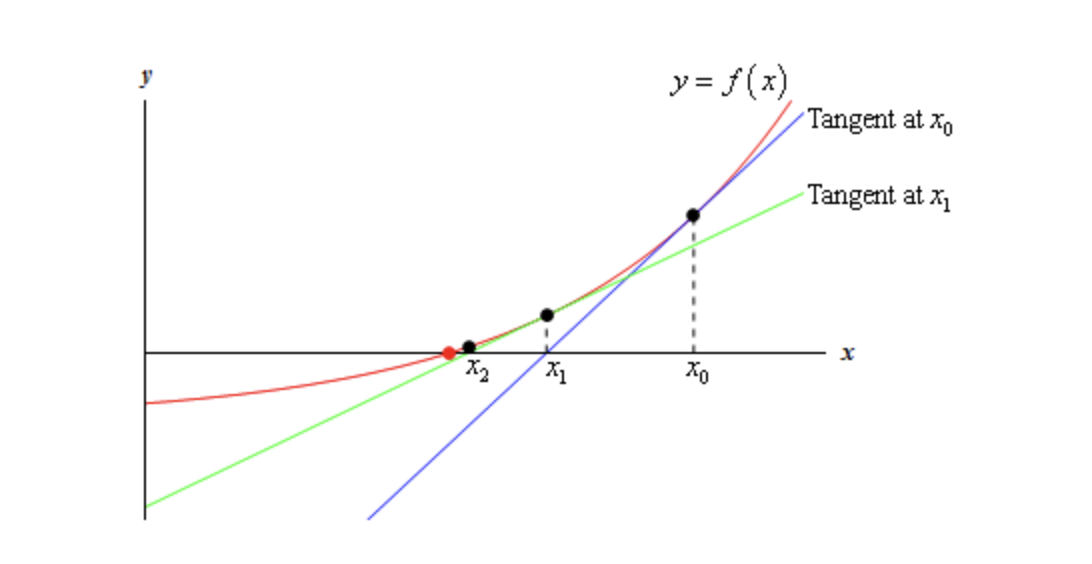
\includegraphics[scale=0.5]{newtonpic}
\end{center}
Thus, Newton's Method can be described by the recursive formula
$$x_{n+1}=x_n-\frac{f(x_n)}{f'(x_n)}.$$
This requires that $f'(x_n)\neq 0$ for all $n$. \\
\vspace{2mm}

\textbf{Project 1:} Using MATLAB, define a function that will do Newton's method for you.  Think about what arguments you want your function to take, and when you want it to terminate (you should probably define some kind of tolerance).  
\vspace{2mm}

\textbf{Project 2:} If a function has more than one root, different initial values will converge to different roots.  Using your code from Project 1, write a script that will create a figure that colors different starting values based on which roots they converge to (create an array, and use imagesc).

\textbf{Project 3:} Doing Newton's Method in the complex plane and coloring based on which roots each initial value will converge to will create fractals! Can you adapt your code from Project 2 to work in the complex plane?  (I'll admit this project is tricky; there's code in the EDGE dropbox if you want a hint.) These types of fractals are known as {\it Julia sets}.  The following pictures are Julia sets generated from the complex function $f(z)=z^8-3z^3+z^2-1$. 
\begin{center}
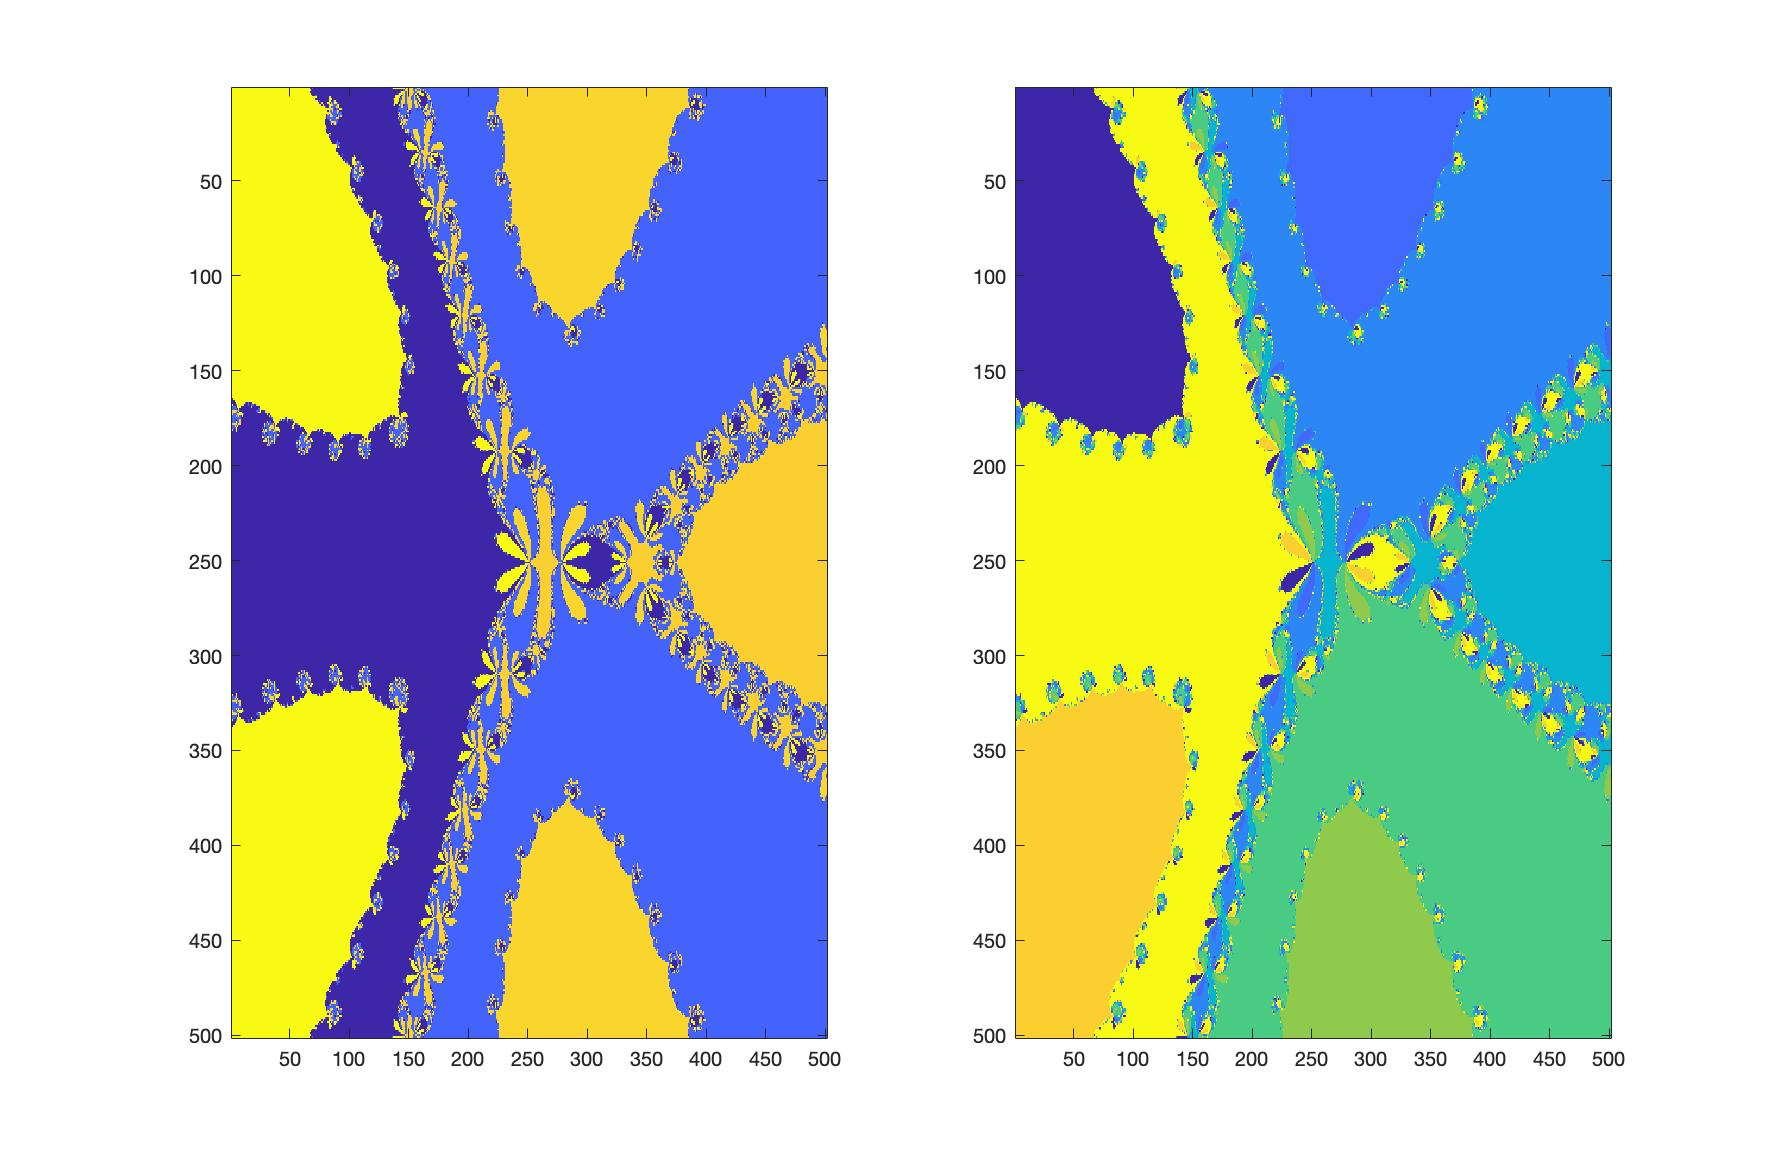
\includegraphics[scale=0.2]{julia.jpg}
\end{center}
\end{document}